%%%%%%%%%%%%%%%%%%%%%%%%%%%%%%%%%%%%%%%%%%%%%%%%%%%%%
%
%  Template
%  Beamer Presentation by Chris Bourke
%
%%%%%%%%%%%%%%%%%%%%%%%%%%%%%%%%%%%%%%%%%%%%%%%%%%%%%%%%%%%%%%%%%%%%%%%

\documentclass[]{beamer}
%\documentclass[handout]{beamer}

\geometry{papersize={16cm,9cm}}

% For handout version:
%\usetheme[hideothersubsections,slidenumbers]{UNLTheme}
\usetheme[hideothersubsections]{UNLTheme}
\usepackage{amssymb}
\input{StandardCommands}
\usepackage[linesnumbered,ruled,vlined]{algorithm2e}
\SetKwComment{Comment}{//}{}
\DontPrintSemicolon
\SetKwSty{textsc} %
%\SetAlFnt{\scriptsize} %
\SetKwInOut{Input}{Input} %
\SetKwInOut{Output}{Output} %
%\setalcapskip{1em} % changed to
\SetAlCapSkip{1em}
\setlength{\algomargin}{2em} %
%\Setvlineskip{0em} % changed to:
\SetVlineSkip{0em}

\usepackage{tikz}
\usetikzlibrary{fadings}
\usetikzlibrary{shapes.geometric,shapes.symbols}
\usetikzlibrary{calc,shapes.multipart,chains,arrows}
\usetikzlibrary{arrows.meta,calc,shapes.multipart,chains,arrows}
%\usetikzlibrary{calc,shapes.multipart,chains,arrows}
%%\usetikzlibrary{backgrounds}
\usetikzlibrary{backgrounds}
\usetikzlibrary{decorations.pathreplacing}
\usetikzlibrary{decorations.pathmorphing}
\tikzset{onslide/.code args={<#1>#2}{%
  \only<#1>{\pgfkeysalso{#2}} % \pgfkeysalso doesn't change the path
}}
\tikzset{temporal/.code args={<#1>#2#3#4}{%
  \temporal<#1>{\pgfkeysalso{#2}}{\pgfkeysalso{#3}}{\pgfkeysalso{#4}} % \pgfkeysalso doesn't change the path
}}


\tikzset{
    fading speed/.code={
        \pgfmathtruncatemacro\tikz@startshading{50-(100-#1)*0.25}
        \pgfmathtruncatemacro\tikz@endshading{50+(100-#1)*0.25}
        \pgfdeclareverticalshading[%
            tikz@axis@top,tikz@axis@middle,tikz@axis@bottom%
        ]{axis#1}{100bp}{%
            color(0bp)=(tikz@axis@bottom);
            color(\tikz@startshading)=(tikz@axis@bottom);
            color(50bp)=(tikz@axis@middle);
            color(\tikz@endshading)=(tikz@axis@top);
            color(100bp)=(tikz@axis@top)
        }
        \tikzset{shading=axis#1}
    }
}

\usepackage{multirow}
\usepackage{multicol}

\definecolor{steelblue}{rgb}{0.2745,0.5098,0.7059}
\definecolor{limegreen}{RGB}{50,205,50}
\hypersetup{
    colorlinks = true,
    urlcolor = {steelblue},
    linkbordercolor = {white}
}

\definecolor{mintedBackground}{rgb}{0.95,0.95,0.95}
\definecolor{mintedInlineBackground}{rgb}{.90,.90,1}

%\usepackage{newfloat}
\usepackage{minted}
\setminted{mathescape,
               linenos,
               autogobble,
               frame=none,
               fontsize=\small,
               framesep=2mm,
               framerule=0.4pt,
               %label=foo,
               xleftmargin=2em,
               xrightmargin=0em,
               startinline=true,  %PHP only, allow it to omit the PHP Tags *** with this option, variables using dollar sign in comments are treated as latex math
               numbersep=10pt, %gap between line numbers and start of line
               style=default, %syntax highlighting style, default is "default"
               			    %gallery: http://help.farbox.com/pygments.html
			    	    %list available: pygmentize -L styles
               bgcolor=mintedBackground} %prevents breaking across pages
               
\setmintedinline{bgcolor={mintedInlineBackground}}
\setminted[text]{bgcolor={},linenos=false,autogobble,xleftmargin=1em}

\tikzstyle{decision} = [diamond, draw, fill=yellow!20, 
    text width=6em, text badly centered, node distance=5cm, inner sep=0pt]
\tikzstyle{block} = [rectangle, draw, fill=blue!20, 
    text width=5em, text centered, node distance=5cm, minimum height=4em]
\tikzstyle{action} = [rectangle, draw, fill=green!20, 
    text width=5em, text centered, rounded corners, node distance=5cm, minimum height=4em]
\tikzstyle{line} = [draw, -latex']

\usepackage{amsmath}

\usepackage{tikz}
\usetikzlibrary{calc,shapes}

\newcommand{\tikzmark}[1]{\tikz[overlay,remember picture] \node (#1) {};}
\newcommand{\DrawBox}[2]{%
  \begin{tikzpicture}[overlay,remember picture]
    \draw[->,shorten >=5pt,shorten <=5pt,out=135,in=45,distance=0.75cm,#1] (MarkC.north) to (MarkA.north);
    \draw[->,shorten >=5pt,shorten <=5pt,out=135,in=45,distance=0.33cm,#2] (MarkC.north) to (MarkB.north);
  \end{tikzpicture}
}

\usetikzlibrary{trees}

% Daniel's proposal for "uncovering" parts of a tikz-tree %
\tikzset{
  invisible/.style={opacity=0},
  visible on/.style={alt=#1{}{invisible}},
  alt/.code args={<#1>#2#3}{%
    \alt<#1>{\pgfkeysalso{#2}}{\pgfkeysalso{#3}} % \pgfkeysalso doesn't change the path
  },
}   

\title[~]{Computer Science I}
\subtitle{Recursion}
\author[~]{Dr.\ Chris Bourke\\ \email{cbourke@cse.unl.edu}} %
\date{~}

\begin{document}

\begin{frame}
  \titlepage
\end{frame}

\setbeamertemplate{section in toc}{\inserttocsectionnumber.~\inserttocsection}
\setbeamercolor{section in toc}{fg=black}
%\setbeamertemplate{subsection in toc}{~} %\inserttocsubsection\\}

\begin{frame}
  \frametitle{Outline}
%{\footnotesize
%\begin{NoHyper}
%  \tableofcontents[hideallsubsections]
%\end{NoHyper}
%}

\setbeamercolor{enumerate item}{bg=white,fg=black}
\setbeamercolor{item}{bg=white,fg=black}
\setbeamercolor{item projected}{bg=white,fg=black}
\setbeamercolor{enumerate subitem}{fg=red!80!black}
\setbeamertemplate{enumerate items}[default]
\begin{enumerate}
  \item Introduction
  \item Designing Recursive Functions
  \item Avoiding Recursion
\end{enumerate}

\end{frame}

\section{Introduction}

\begin{frame}
    \frametitle{}
    \framesubtitle{}
    
    \begin{center}
    {\Huge Part I: Introduction}\\
    {\Large ~}
    \end{center}

\end{frame}

\begin{frame}[fragile]
  \frametitle{Challenge}
  \framesubtitle{}

Challenge: write code to count down from 10 to 1 
\emph{without} using a loop.

\end{frame}


\begin{frame}[fragile]
  \frametitle{Challenge}
  \framesubtitle{}

\begin{minted}{c}
void countDown(int n) {

  if(n < 0) {
    printf("Error: cannot count down from negatives!");
  } else if(n == 0) {
    printf("Blast Off\n");
  } else {
    printf("%d\n", n);
    countDown(n-1);
  }
  return;
}
\end{minted}

\end{frame}

\begin{frame}[fragile]
  \frametitle{Recursion}
  \framesubtitle{}

\begin{itemize}[<+->]
  \item \emph{Recursion} is when something is defined in terms of itself
  \item Mathematics: recurrence relations, Fibonacci Sequence
    $$F(n) = \left\{\begin{array}{ll}
    1 & \textrm{if } n = 1 \\
    1 & \textrm{if } n = 2 \\
    F(n-1) + F(n-2) & \textrm{otherwise}
    \end{array}\right.$$
  \item[~]
\begin{equation}
1, \,\, 1,\,\, 2,\,\, 3,\,\, 5,\,\, 8,\,\, 13,\,\,  2\tikzmark{MarkA}1,\,\,  3\tikzmark{MarkB}4,\,\,  5\tikzmark{MarkC}5\DrawBox{black}{black}
\end{equation}

  \end{itemize}


\end{frame}

\begin{frame}[fragile]
  \frametitle{Fractals}
  \framesubtitle{}

\begin{center}
\includegraphics[scale=0.65]{serpinskiTriangles}

Serpinski Triangles
\end{center}

\end{frame}

\begin{frame}[fragile]
  \frametitle{Fractals}
  \framesubtitle{}

\begin{center}
\includegraphics[scale=0.15]{bay}

Mandelbrot Set
\end{center}

\end{frame}

\begin{frame}[fragile]
  \frametitle{Recursive Functions}
  \framesubtitle{}

\begin{itemize}[<+->]
  \item A \emph{recursive function} is a function that makes one or more
  ``recursive calls'' to itself
  \item Generally recursive calls pass in different parameter values
  %\item Can ``simulate'' loop control structures
  \item More generally: divide-and-conquer style problem solving
\end{itemize}

\end{frame}

\section{Writing Recursively}

\begin{frame}
    \frametitle{}
    \framesubtitle{}
    
    \begin{center}
    {\Huge Part II: Writing Recursive Functions}\\
    {\Large ~}
    \end{center}

\end{frame}

\begin{frame}[fragile]
  \frametitle{Recursion}
  \framesubtitle{}

In general, every recursive function must have:
\begin{enumerate}[<+->]
  \item A \emph{base case} -- a condition after which the recursion stops
  \item Each recursive call must make progress toward the base case
  \item Corner cases may need to be handled separately 
\end{enumerate}

\end{frame}

\begin{frame}[fragile]
  \frametitle{Thinking Recursively}
  \framesubtitle{}

\begin{itemize}[<+->]
  \item A recursive solution requires you to think about a general ``case''
  \item Similar to loops: at the $i$-th iteration what do you do?
  \item Given the input, how do you \emph{divide-and-conquer} it?
\end{itemize}

\end{frame}


\begin{frame}[fragile]
  \frametitle{Examples}
  \framesubtitle{}

\begin{itemize}[<+->]
  \item Write a recursive function to compute the fibonacci sequence
  \item Write a recursive function to find the largest element in an array
  of integers (simulate a traditional loop)
  \item Write a recursive, \emph{divide-and-conquer}-style function to
  sum the elements in an array of integers
\end{itemize}

\end{frame}

\begin{frame}[fragile]
  \frametitle{Fibonacci Solution}
  \framesubtitle{}

\begin{minted}{c}
int fibonacci(int n) {

  if(n < 1) {
    return -1;
  } else if(n == 1 || n == 2) {
    return 1;
  } else {
    return fibonacci(n-1) + fibonacci(n-2);
  }

}
\end{minted}

\end{frame}


\begin{frame}[fragile]
  \frametitle{Largest Element Solution}
  \framesubtitle{}

\begin{minted}{c}
int largestElement(const int *arr, int largest, int index) {
  if(index < 0) {
    return largest;
  } else {
    if(arr[index] > largest) {
      return largestElement(arr, arr[index], index-1);
    } else {
      return largestElement(arr, largest, index-1);      
    }
  }
}
\end{minted}

\end{frame}


\begin{frame}[fragile]
  \frametitle{Summation Solution}
  \framesubtitle{}

\begin{minted}{c}
int recursiveSum(const int *arr, int l, int r) {
  if(l > r) {
    return 0;
  } else if(l == r) {
    return arr[l];
  } else {
    int m = (l + r) / 2;
    return recursiveSum(arr, l, m) + recursiveSum(arr, m+1, r);      
  }
}
\end{minted}

\end{frame}


\begin{frame}[fragile]
  \frametitle{Divide \& Conquer}
  \framesubtitle{}

\begin{center}
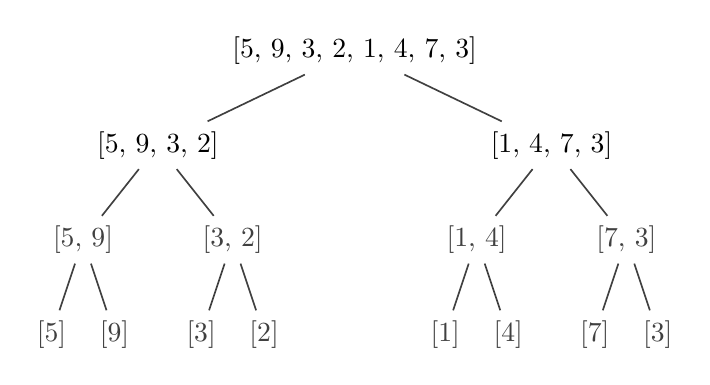
\begin{tikzpicture}[
ball/.style={circle, thick, solid,inner sep=0.5mm, minimum size=5mm},
nor/.style={ball,draw=black,fill=none},
acc/.style={ball,draw=green!50!black,fill=green!20},
rej/.style={ball,draw=red!50,fill=red!20},
level 1/.style={sibling distance=50mm,every child/.style={edge from parent/.style={solid,draw,nearly opaque, visible on=<2->}}},
level 2/.style={sibling distance=19mm,every child/.style={edge from parent/.style={solid,draw,visible on=<2->}}},
level 3/.style={sibling distance=8mm },
semithick]

\node[draw=none] (root) {[5, 9, 3, 2, 1, 4, 7, 3]}
  child[level distance=12mm,visible on=<2->] { node[] {[5, 9, 3, 2]}    
    child[level distance=12mm,visible on=<3->] { node[] {[5, 9]}    
      child[level distance=12mm,visible on=<4->] { node[] {[5]}    
      }
      child[level distance=12mm,visible on=<4->] { node[] {[9]}    
      }
    }
    child[level distance=12mm,visible on=<3->] { node[] {[3, 2]}    
      child[level distance=12mm,visible on=<4->] { node[] {[3]}    
      }
      child[level distance=12mm,visible on=<4->] { node[] {[2]}    
      }
    }
  }
  child[level distance=12mm,visible on=<2->] { node[] {[1, 4, 7, 3]} 
    child[level distance=12mm,visible on=<3->] { node[] {[1, 4]}    
      child[level distance=12mm,visible on=<4->] { node[] {[1]}    
      }
      child[level distance=12mm,visible on=<4->] { node[] {[4]}    
      }
    }
    child[level distance=12mm,visible on=<3->] { node[] {[7, 3]}    
      child[level distance=12mm,visible on=<4->] { node[] {[7]}    
      }
      child[level distance=12mm,visible on=<4->] { node[] {[3]}    
      }
    }
  }
;
\end{tikzpicture}
\end{center}  
\end{frame}

\begin{frame}[fragile]
  \frametitle{Divide \& Conquer}
  \framesubtitle{}%2

\begin{center}
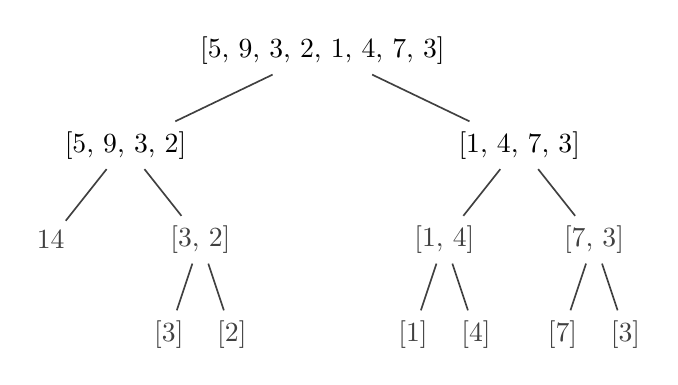
\begin{tikzpicture}[
ball/.style={circle, thick, solid,inner sep=0.5mm, minimum size=5mm},
nor/.style={ball,draw=black,fill=none},
acc/.style={ball,draw=green!50!black,fill=green!20},
rej/.style={ball,draw=red!50,fill=red!20},
level 1/.style={sibling distance=50mm,every child/.style={edge from parent/.style={solid,draw,nearly opaque, visible on=<1->}}},
level 2/.style={sibling distance=19mm,every child/.style={edge from parent/.style={solid,draw,visible on=<1->}}},
level 3/.style={sibling distance=8mm },
semithick]

\node[draw=none] (root) {[5, 9, 3, 2, 1, 4, 7, 3]}
  child[level distance=12mm,visible on=<1->] { node[] {[5, 9, 3, 2]}    
    child[level distance=12mm,visible on=<1->] { node[] {14}    
    }
    child[level distance=12mm,visible on=<1->] { node[] {[3, 2]}    
      child[level distance=12mm,visible on=<1->] { node[] {[3]}    
      }
      child[level distance=12mm,visible on=<1->] { node[] {[2]}    
      }
    }
  }
  child[level distance=12mm,visible on=<1->] { node[] {[1, 4, 7, 3]} 
    child[level distance=12mm,visible on=<1->] { node[] {[1, 4]}    
      child[level distance=12mm,visible on=<1->] { node[] {[1]}    
      }
      child[level distance=12mm,visible on=<1->] { node[] {[4]}    
      }
    }
    child[level distance=12mm,visible on=<1->] { node[] {[7, 3]}    
      child[level distance=12mm,visible on=<1->] { node[] {[7]}    
      }
      child[level distance=12mm,visible on=<1->] { node[] {[3]}    
      }
    }
  }
;
\end{tikzpicture}
\end{center}  
\end{frame}

\begin{frame}[fragile]
  \frametitle{Divide \& Conquer}
  \framesubtitle{}%3

\begin{center}
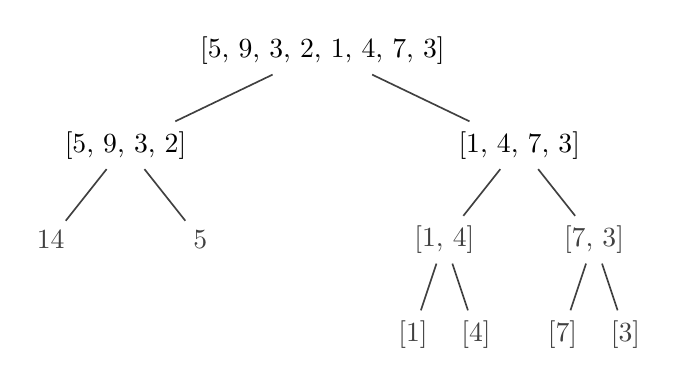
\begin{tikzpicture}[
ball/.style={circle, thick, solid,inner sep=0.5mm, minimum size=5mm},
nor/.style={ball,draw=black,fill=none},
acc/.style={ball,draw=green!50!black,fill=green!20},
rej/.style={ball,draw=red!50,fill=red!20},
level 1/.style={sibling distance=50mm,every child/.style={edge from parent/.style={solid,draw,nearly opaque, visible on=<1->}}},
level 2/.style={sibling distance=19mm,every child/.style={edge from parent/.style={solid,draw,visible on=<1->}}},
level 3/.style={sibling distance=8mm },
semithick]

\node[draw=none] (root) {[5, 9, 3, 2, 1, 4, 7, 3]}
  child[level distance=12mm,visible on=<1->] { node[] {[5, 9, 3, 2]}    
    child[level distance=12mm,visible on=<1->] { node[] {14}    
    }
    child[level distance=12mm,visible on=<1->] { node[] {5}    
    }
  }
  child[level distance=12mm,visible on=<1->] { node[] {[1, 4, 7, 3]} 
    child[level distance=12mm,visible on=<1->] { node[] {[1, 4]}    
      child[level distance=12mm,visible on=<1->] { node[] {[1]}    
      }
      child[level distance=12mm,visible on=<1->] { node[] {[4]}    
      }
    }
    child[level distance=12mm,visible on=<1->] { node[] {[7, 3]}    
      child[level distance=12mm,visible on=<1->] { node[] {[7]}    
      }
      child[level distance=12mm,visible on=<1->] { node[] {[3]}    
      }
    }
  }
;
\end{tikzpicture}
\end{center}  
\end{frame}

\begin{frame}[fragile]
  \frametitle{Divide \& Conquer}
  \framesubtitle{}%4

\begin{center}
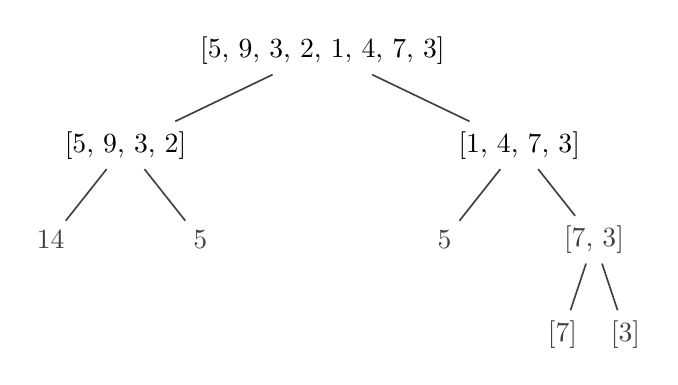
\begin{tikzpicture}[
ball/.style={circle, thick, solid,inner sep=0.5mm, minimum size=5mm},
nor/.style={ball,draw=black,fill=none},
acc/.style={ball,draw=green!50!black,fill=green!20},
rej/.style={ball,draw=red!50,fill=red!20},
level 1/.style={sibling distance=50mm,every child/.style={edge from parent/.style={solid,draw,nearly opaque, visible on=<1->}}},
level 2/.style={sibling distance=19mm,every child/.style={edge from parent/.style={solid,draw,visible on=<1->}}},
level 3/.style={sibling distance=8mm },
semithick]

\node[draw=none] (root) {[5, 9, 3, 2, 1, 4, 7, 3]}
  child[level distance=12mm,visible on=<1->] { node[] {[5, 9, 3, 2]}    
    child[level distance=12mm,visible on=<1->] { node[] {14}    
    }
    child[level distance=12mm,visible on=<1->] { node[] {5}    
    }
  }
  child[level distance=12mm,visible on=<1->] { node[] {[1, 4, 7, 3]} 
    child[level distance=12mm,visible on=<1->] { node[] {5}    
    }
    child[level distance=12mm,visible on=<1->] { node[] {[7, 3]}    
      child[level distance=12mm,visible on=<1->] { node[] {[7]}    
      }
      child[level distance=12mm,visible on=<1->] { node[] {[3]}    
      }
    }
  }
;
\end{tikzpicture}
\end{center}  
\end{frame}

\begin{frame}[fragile]
  \frametitle{Divide \& Conquer}
  \framesubtitle{}%5

\begin{center}
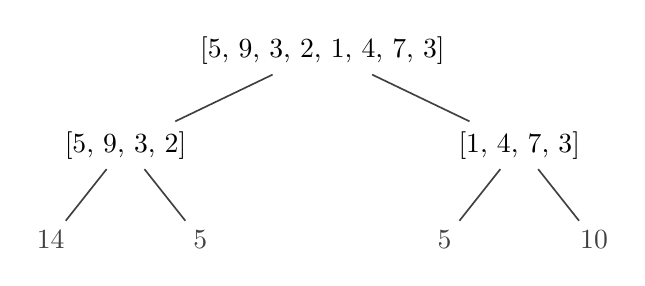
\begin{tikzpicture}[
ball/.style={circle, thick, solid,inner sep=0.5mm, minimum size=5mm},
nor/.style={ball,draw=black,fill=none},
acc/.style={ball,draw=green!50!black,fill=green!20},
rej/.style={ball,draw=red!50,fill=red!20},
level 1/.style={sibling distance=50mm,every child/.style={edge from parent/.style={solid,draw,nearly opaque, visible on=<1->}}},
level 2/.style={sibling distance=19mm,every child/.style={edge from parent/.style={solid,draw,visible on=<1->}}},
level 3/.style={sibling distance=8mm },
semithick]

\node[draw=none] (root) {[5, 9, 3, 2, 1, 4, 7, 3]}
  child[level distance=12mm,visible on=<1->] { node[] {[5, 9, 3, 2]}    
    child[level distance=12mm,visible on=<1->] { node[] {14}    
    }
    child[level distance=12mm,visible on=<1->] { node[] {5}    
    }
  }
  child[level distance=12mm,visible on=<1->] { node[] {[1, 4, 7, 3]} 
    child[level distance=12mm,visible on=<1->] { node[] {5}
    }
    child[level distance=12mm,visible on=<1->] { node[] {10}    
    }
  }
;
\end{tikzpicture}
\end{center}  
\end{frame}

\begin{frame}[fragile]
  \frametitle{Divide \& Conquer}
  \framesubtitle{}%6

\begin{center}
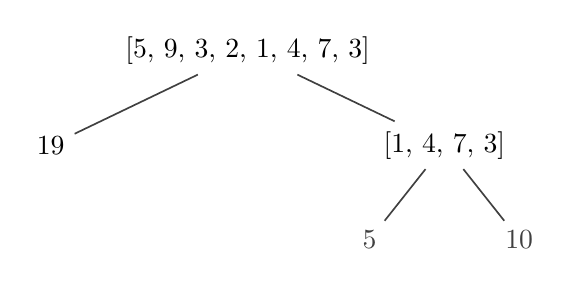
\begin{tikzpicture}[
ball/.style={circle, thick, solid,inner sep=0.5mm, minimum size=5mm},
nor/.style={ball,draw=black,fill=none},
acc/.style={ball,draw=green!50!black,fill=green!20},
rej/.style={ball,draw=red!50,fill=red!20},
level 1/.style={sibling distance=50mm,every child/.style={edge from parent/.style={solid,draw,nearly opaque, visible on=<1->}}},
level 2/.style={sibling distance=19mm,every child/.style={edge from parent/.style={solid,draw,visible on=<1->}}},
level 3/.style={sibling distance=8mm },
semithick]

\node[draw=none] (root) {[5, 9, 3, 2, 1, 4, 7, 3]}
  child[level distance=12mm,visible on=<1->] { node[] {19}    
  }
  child[level distance=12mm,visible on=<1->] { node[] {[1, 4, 7, 3]} 
    child[level distance=12mm,visible on=<1->] { node[] {5}
    }
    child[level distance=12mm,visible on=<1->] { node[] {10}    
    }
  }
;
\end{tikzpicture}
\end{center}  
\end{frame}

\begin{frame}[fragile]
  \frametitle{Divide \& Conquer}
  \framesubtitle{}%7

\begin{center}
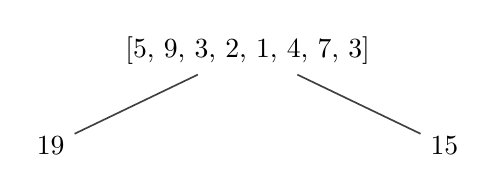
\begin{tikzpicture}[
ball/.style={circle, thick, solid,inner sep=0.5mm, minimum size=5mm},
nor/.style={ball,draw=black,fill=none},
acc/.style={ball,draw=green!50!black,fill=green!20},
rej/.style={ball,draw=red!50,fill=red!20},
level 1/.style={sibling distance=50mm,every child/.style={edge from parent/.style={solid,draw,nearly opaque, visible on=<1->}}},
level 2/.style={sibling distance=19mm,every child/.style={edge from parent/.style={solid,draw,visible on=<1->}}},
level 3/.style={sibling distance=8mm },
semithick]

\node[draw=none] (root) {[5, 9, 3, 2, 1, 4, 7, 3]}
  child[level distance=12mm,visible on=<1->] { node[] {19}    
  }
  child[level distance=12mm,visible on=<1->] { node[] {15} 
  }
;
\end{tikzpicture}
\end{center}  
\end{frame}

\begin{frame}[fragile]
  \frametitle{Divide \& Conquer}
  \framesubtitle{}%7

\begin{center}
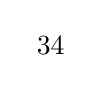
\begin{tikzpicture}[
ball/.style={circle, thick, solid,inner sep=0.5mm, minimum size=5mm},
nor/.style={ball,draw=black,fill=none},
acc/.style={ball,draw=green!50!black,fill=green!20},
rej/.style={ball,draw=red!50,fill=red!20},
level 1/.style={sibling distance=50mm,every child/.style={edge from parent/.style={solid,draw,nearly opaque, visible on=<1->}}},
level 2/.style={sibling distance=19mm,every child/.style={edge from parent/.style={solid,draw,visible on=<1->}}},
level 3/.style={sibling distance=8mm },
semithick]

\node[draw=none] (root) {34};
\end{tikzpicture}
\end{center}  
\end{frame}

\section{Avoiding Recursion}

\begin{frame}
    \frametitle{}
    \framesubtitle{}
    
    \begin{center}
    {\Huge Part III: Avoiding Recursion}\\
    {\Large ~}
    \end{center}

\end{frame}


\begin{frame}[fragile]
  \frametitle{Recursion: Advantages}
  \framesubtitle{}
    
\begin{itemize}[<+->]
  \item Recursion can be a useful problem solving technique
  \item Divide \& Conquer strategies are generally presented as recursive
  \item Functional programming languages (Lisp, Haskell) use recursion as a
  fundamental control flow mechanism
%  \item Functional/recursive style is more inline with ``mathematical thinking''
\end{itemize}    

\end{frame}

\begin{frame}[fragile]
  \frametitle{Recursion: Disadvantages}
  \framesubtitle{}
    
\begin{itemize}[<+->]
  \item In practice, recursion is not necessary: any (computable)
    recursive function can be rewritten using a loop and/or smart data structure
  \item Many style guides discourage or forbid the use of recursion
  %especially in embedded systems
  \item Recursive functions can ``abuse'' the program stack by creating 
  and destroying many stack frames
  \item Deep recursion risks \emph{stack overflow}%: demo this on visualizer  
  \item Demonstration
\end{itemize} 

\end{frame}


\begin{frame}[fragile]
  \frametitle{Recursion: Disadvantages}
  \framesubtitle{}
    
\begin{itemize}[<+->]
  \item Recursion can be extremely inefficient when not done properly
  \item Perfect example: Fibonacci code
  \item The same computations are performed over and over multiple times
  \item Computation Tree
\end{itemize} 

\end{frame}


\begin{frame}[fragile]
  \frametitle{Computation Tree}
  \framesubtitle{}

\begin{center}    
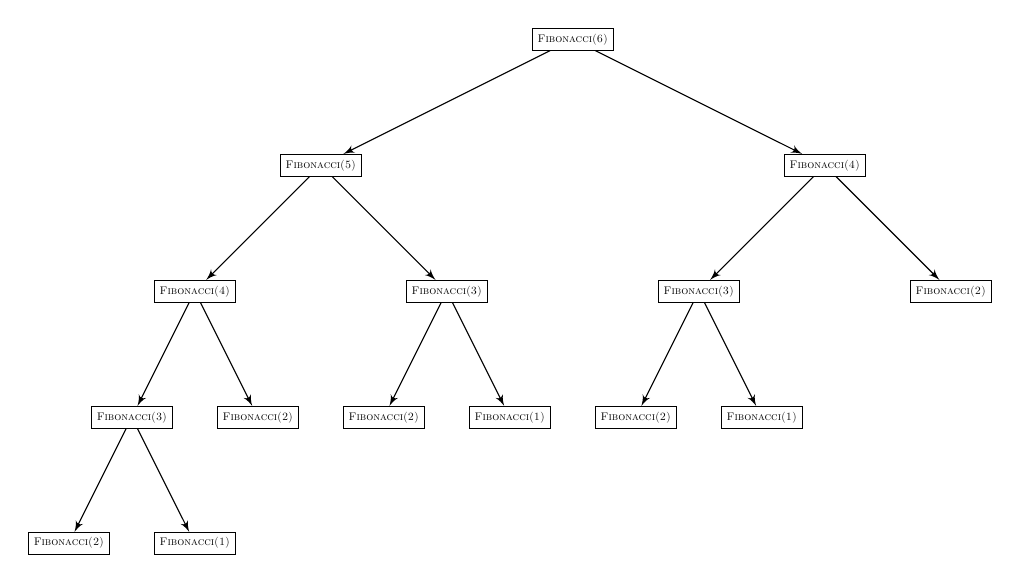
\begin{tikzpicture}
  [scale=.40,transform shape,
   level distance=4cm,
   every node/.style={rectangle,
                      thin,
                      draw=black,
                      %top color = white,
                      %bottom color = black!50,
                      inner sep=5pt,
                      %drop shadow={opacity=0.35,shadow xshift=.2ex, shadow yshift=-.2ex}
                      },
   edge from parent/.style={->,draw,>=latex'},
   level 1/.style={sibling distance=16cm},
   level 2/.style={sibling distance=8cm},
   level 3/.style={sibling distance=4cm},
   level 4/.style={sibling distance=4cm}]
  \node {\textsc{Fibonacci(6)}}
     child {node {\textsc{Fibonacci(5)}}
       child {node {\textsc{Fibonacci(4)}}
         child {node {\textsc{Fibonacci(3)}}
          child {node {\textsc{Fibonacci(2)}}}
          child {node {\textsc{Fibonacci(1)}}}
         }
         child {node {\textsc{Fibonacci(2)}}}
       }
       child {node {\textsc{Fibonacci(3)}}
          child {node {\textsc{Fibonacci(2)}}}
          child {node {\textsc{Fibonacci(1)}}}
       }
     }
     child {node {\textsc{Fibonacci(4)}}
        child {node {\textsc{Fibonacci(3)}}
          child {node {\textsc{Fibonacci(2)}}}
          child {node {\textsc{Fibonacci(1)}}}
        }
        child {node {\textsc{Fibonacci(2)}}}
     };
\end{tikzpicture}
\end{center}

\end{frame}


\begin{frame}[fragile]
  \frametitle{Mitigating Problems with Recursion}
  \framesubtitle{}
    
\begin{itemize}[<+->]
  %\item In practice, many algorithms \emph{simulate} recursion 
  \item Alternative solution: \emph{memoization}
  \item Cache values so they can be reused (and not recomputed)
  \item Each recursive call checks to see if the value has been computed
  \item If yes: use it (avoid further recursion)
  \item If no: pay for the recursion, but store the answer
  \item Demonstration
\end{itemize} 

\end{frame}



\end{document} 
